% SIAM Shared Information Template
% This is information that is shared between the main document and any
% supplement. If no supplement is required, then this information can
% be included directly in the main document.

As pointed out previously, the parallelization of
the \acrshort{SymmSpMV} kernel can be done
via \DTWO coloring of the corresponding graph. The computational
intensity, and hence the performance, depends on the data access
patterns to the LHS and RHS vectors. As coloring schemes change those
patterns, they may change the computational intensity, and we have to
investigate this effect in more detail. We apply the basic
\acrshort{MC} scheme generated by COLPACK~\cite{COLPACK} to
parallelize \acrshort{SymmSpMV} and compare it with \acrshort{SpMV},
which serves as our performance yardstick. Note that any required
preprocessing is excluded from the timings. In~\cref{fig:motivation}
we present performance and data transfer volumes for
the \emph{Spin-26} matrix on a single socket of the \IVB
and \SKX systems. For \acrshort{SpMV} we recover the well-known memory bandwidth
saturation pattern as we fill the chip (\cref{fig:motivation_symm_spmv,fig:motivation_symm_spmv_skx}).
 Measuring the actual data volume from main memory using \LIKWID
we find $16.24$ and $16.36$ \BYTE per nonzero matrix entry (\cref{fig:motivation_data,fig:motivation_data_skx})
on \IVB and \SKX architectures.
 This corresponds to the denominator of
$I_\mathrm{\acrshort{SpMV}}$ in~\cref{eq:SpMV_intensity}, so we can
determine $\alpha_\mathrm{\acrshort{SpMV}}=0.351$ for \IVB and $0.367$ for \SKX, thus we can calculate an 
optimistic bound for the intensity of \acrshort{SymmSpMV} according to ~\cref{eq:SymmSpMV_intensity}.
 Using the copy and the load-only bandwidth of \IVB (see~\cref{tab:test_bed}) 
 in \cref{eq:upper_performance} we find a maximum
attainable {\acrshort{SymmSpMV}} performance range for this matrix of
$P_\mathrm{\acrshort{SymmSpMV}}=7.63,\ldots,8.96\,\GF$, while for \SKX we expect  $P_\mathrm{\acrshort{SymmSpMV}}=19.49,\ldots,21.55\,\GF$ . This indicates a possible
speedup of approximately 1.4$\times$ -- 1.6$\times$ compared to the \acrshort{SpMV}
baseline ($5.5\,\GF$ and $13.41\,\GF$ on \IVB and \SKX), the \acrshort{SymmSpMV} implementation
using \acrshort{MC} falls short of this expectation and is more than
three times slower than \acrshort{SpMV}.
\begin{figure}[tbp]
  	\centering
 % 	\subfloat[\acrshort{SpMV}]{\label{fig:motivation_spmv}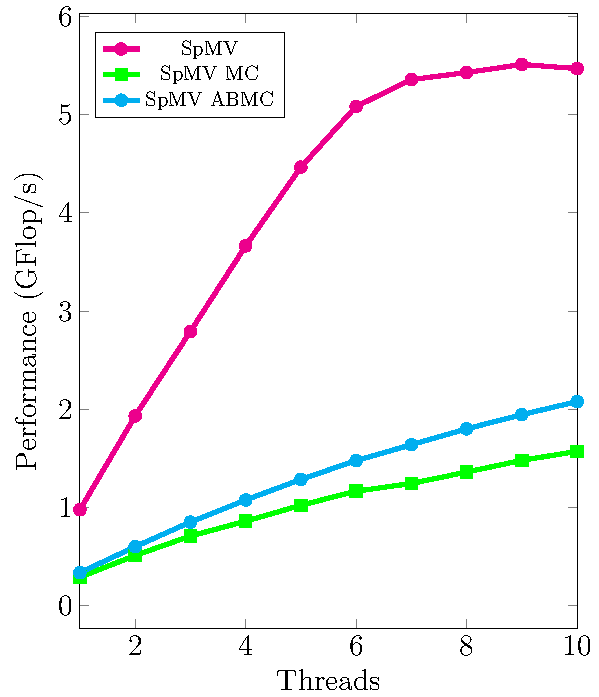
\includegraphics[width=0.26\textwidth, height=0.22\textheight]{pics/motivation/out/motivation_spmv}}
  %	\hspace{1em}
    \subfloat[SymmSpMV]{\label{fig:motivation_symm_spmv}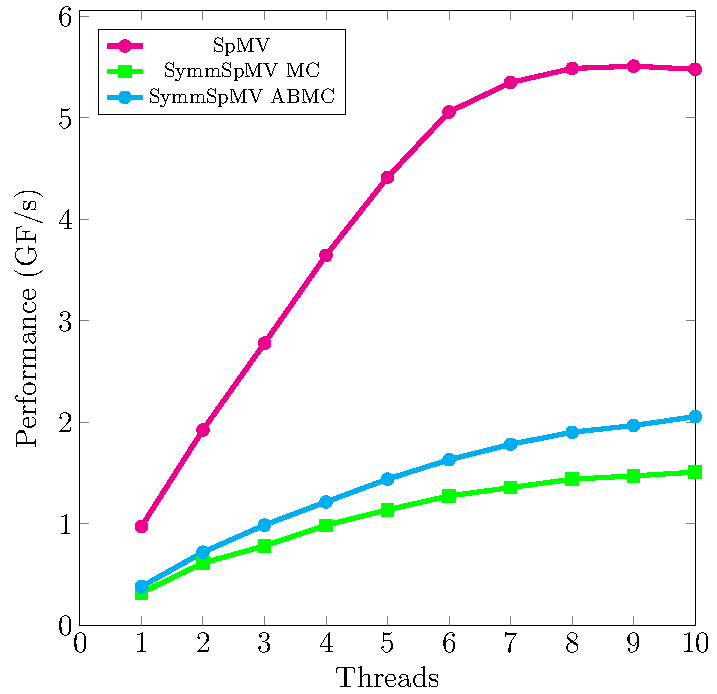
\includegraphics[width=0.248\textwidth, height=0.20\textheight]{pics/motivation/out/motivation_symm_spmv}}
   % \hspace{1em}
  	\subfloat[Data traffic]{\label{fig:motivation_data}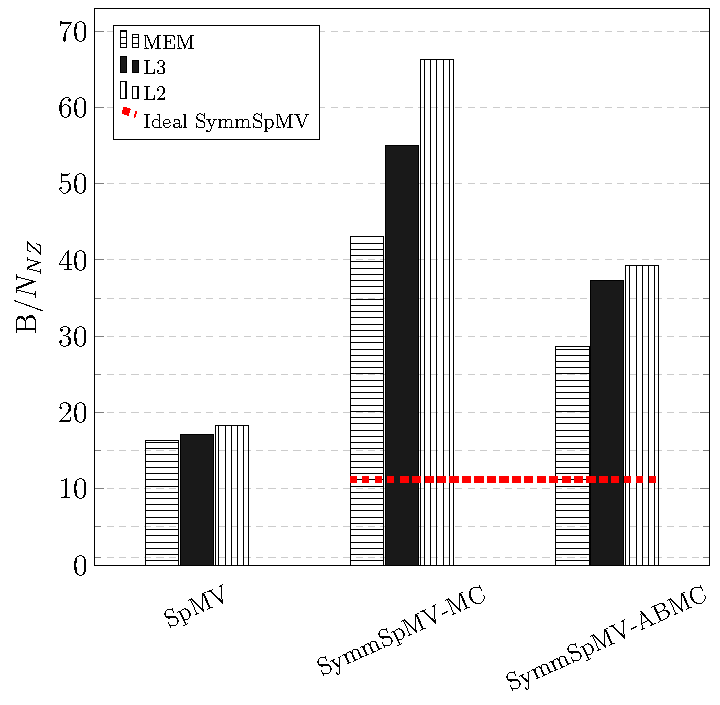
\includegraphics[width=0.248\textwidth, height=0.20\textheight]{pics/motivation/out/motivation_data_wo_RACE}} 
    \subfloat[SymmSpMV]{\label{fig:motivation_symm_spmv_skx}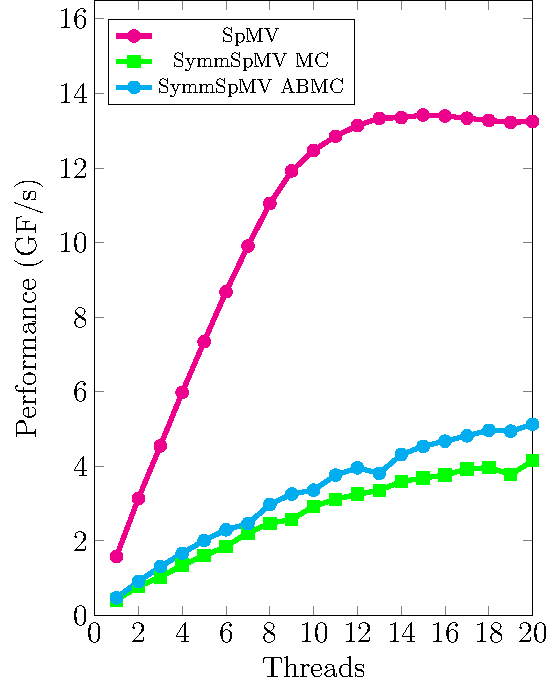
\includegraphics[width=0.248\textwidth, height=0.20\textheight]{pics/motivation/out_skx/motivation_symm_spmv}}
    %\hspace{1em}
    \subfloat[Data traffic]{\label{fig:motivation_data_skx}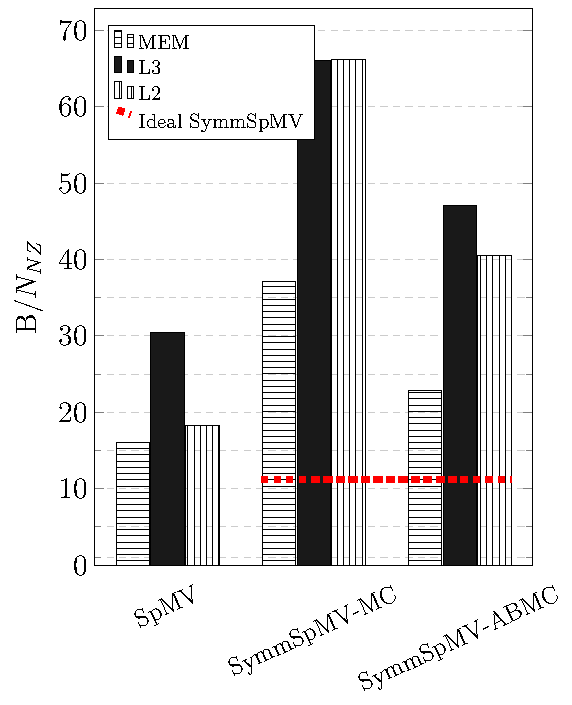
\includegraphics[width=0.248\textwidth, height=0.20\textheight]{pics/motivation/out_skx/motivation_data_wo_RACE}}
  %	\subfloat[False sharing]{\label{fig:motivation_c}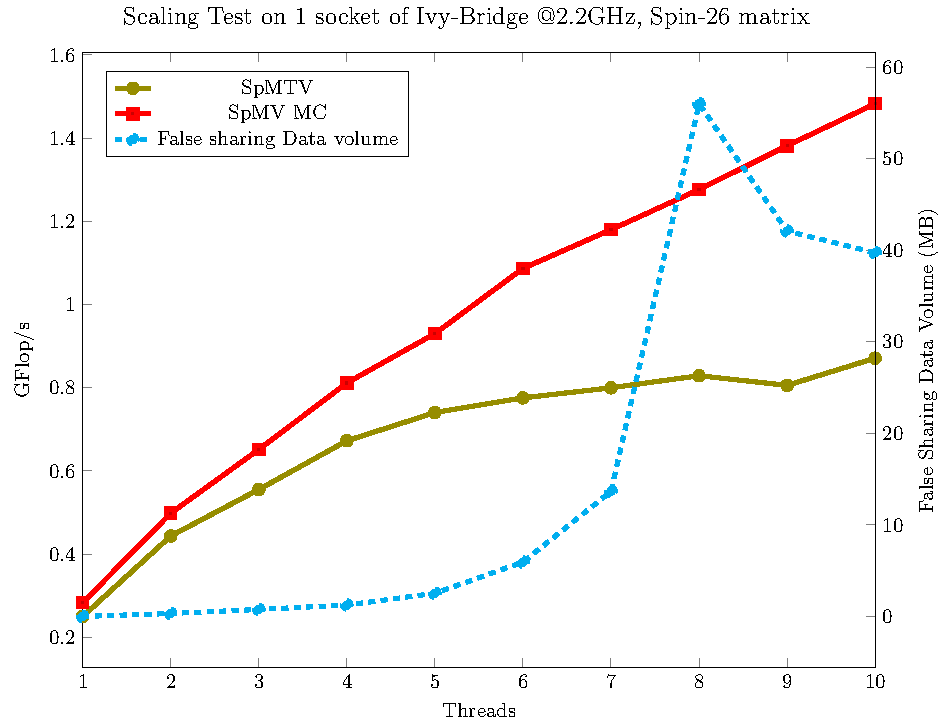
\includegraphics[width=0.45\textwidth, height=0.22\textheight]{pics/motivation/motivation_2}}
  %	\hspace{1em}
  %	\subfloat[Barrier effect]{\label{fig:motivation_d}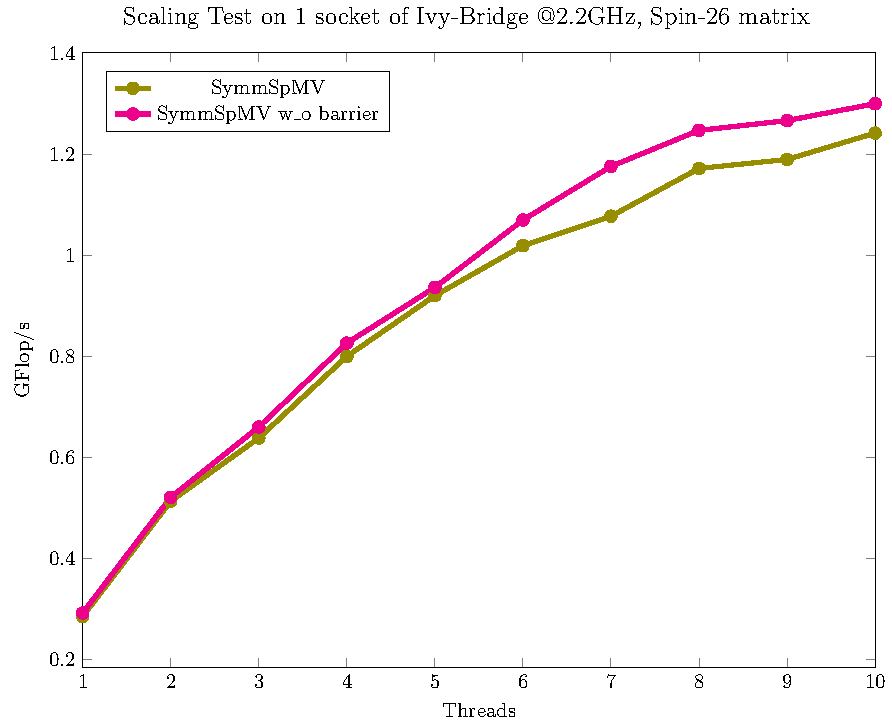
\includegraphics[width=0.45\textwidth, height=0.22\textheight]{pics/motivation/motivation_4}}
  	\caption{Scaling performance of \acrshort{SymmSpMV} with \acrshort{MC} and \acrshort{ABMC} compared to \acrshort{SpMV} on one socket of \IVB and \SKX is shown in \cref{fig:motivation_symm_spmv,fig:motivation_symm_spmv_skx} respectively. \cref{fig:motivation_data,fig:motivation_data_skx} show average data traffic per nonzero entry ($\acrshort{nnz}$) of the full matrix as measured with \LIKWID for all cache levels and main memory on full socket of \IVB and \SKX respectively. The Spin-26 matrix was prepermuted with \acrshort{RCM}. \CAcomm{Note that the L3 measurement on \SKX architecture is qualitative as some performance counter events are missing for the architecture.} }
  	\label{fig:motivation}
  \end{figure}
 
\begin{comment}
{\GW Original Text - bitte auskommentieren
Motivation for developing an alternative method stems from the ESSEX (Equipping Sparse Solvers for Exascale) project \cite{ESSEX}
 where we investigate into solving large eigen-value problems from quantum mechanics field. In this context having a robust iterative solver was inevitable, due to the poor condition number of the matrices that appear in this field. Kaczmarz (\KACZ) solver was found to be satisfactory but parallelizing this solver was deemed challenging because of the loop-carried dependencies in the kernel. Previous work on parallelizing the \KACZ kernel used \acrshort{MC}full (\acrshort{MC}) \cite{feast_mc} but it was soon found that the kernels do not scale efficiently with this approach.
In order to get a better understanding of the underlying problem it's convenient to choose simple symmetric sparse matrix vector (\acrshort{SymmSpMV}) as a benchmark kernel. The particular choice of this kernel is due to the fact that both \KACZ and \acrshort{SymmSpMV} have similar kind of dependencies, and it's much easier to compare with our reference kernel namely sparse matrix vector (\\acrshort{SpMV}) which is embarrassingly parallel. The algorithm for \acrshort{SymmSpMV}  and \\acrshort{SpMV} has been listed in \cref{alg:Symm\acrshort{SpMV},alg:\acrshort{SpMV}}}
 \Cref{fig:motivation_spmv} shows the performance of \\acrshort{SpMV} kernel on original unpermuted matrix and matrix with \acrshort{MC} permutation. Here we see the performance of \\acrshort{SpMV} on multicolored matrix is  four times  worse than that of  \\acrshort{SpMV} on unpermuted matrix. One of the major reason for this drop is due to the increase in $\alpha$ factor seen in the intensity equation \cref{eq:\acrshort{SpMV}_intensity}  Since the kernels like \\acrshort{SpMV}  are mainly memory bound increase in $\alpha$ lowers intensity $I_\mathrm{\\acrshort{SpMV}}$ leading to a drop of performance as predicted by \roofline model \cite{Williams_roofline}. This could easily be demonstrated by measuring the data traffic between different memory hierarchies.  We do this using the \LIKWID tool \cite{LIKWID}, and the measurements can be seen in \cref{fig:motivation_data}. One can see an increase in data-traffic from all the memory hierarchy compared to \\acrshort{SpMV} on normal unpermuted matrix. This is basically caused by the bad data locality introduced by \acrshort{MC}full permutation.
\end{comment}
%  \begin{figure}[htbp]
 % 	\centering
  %	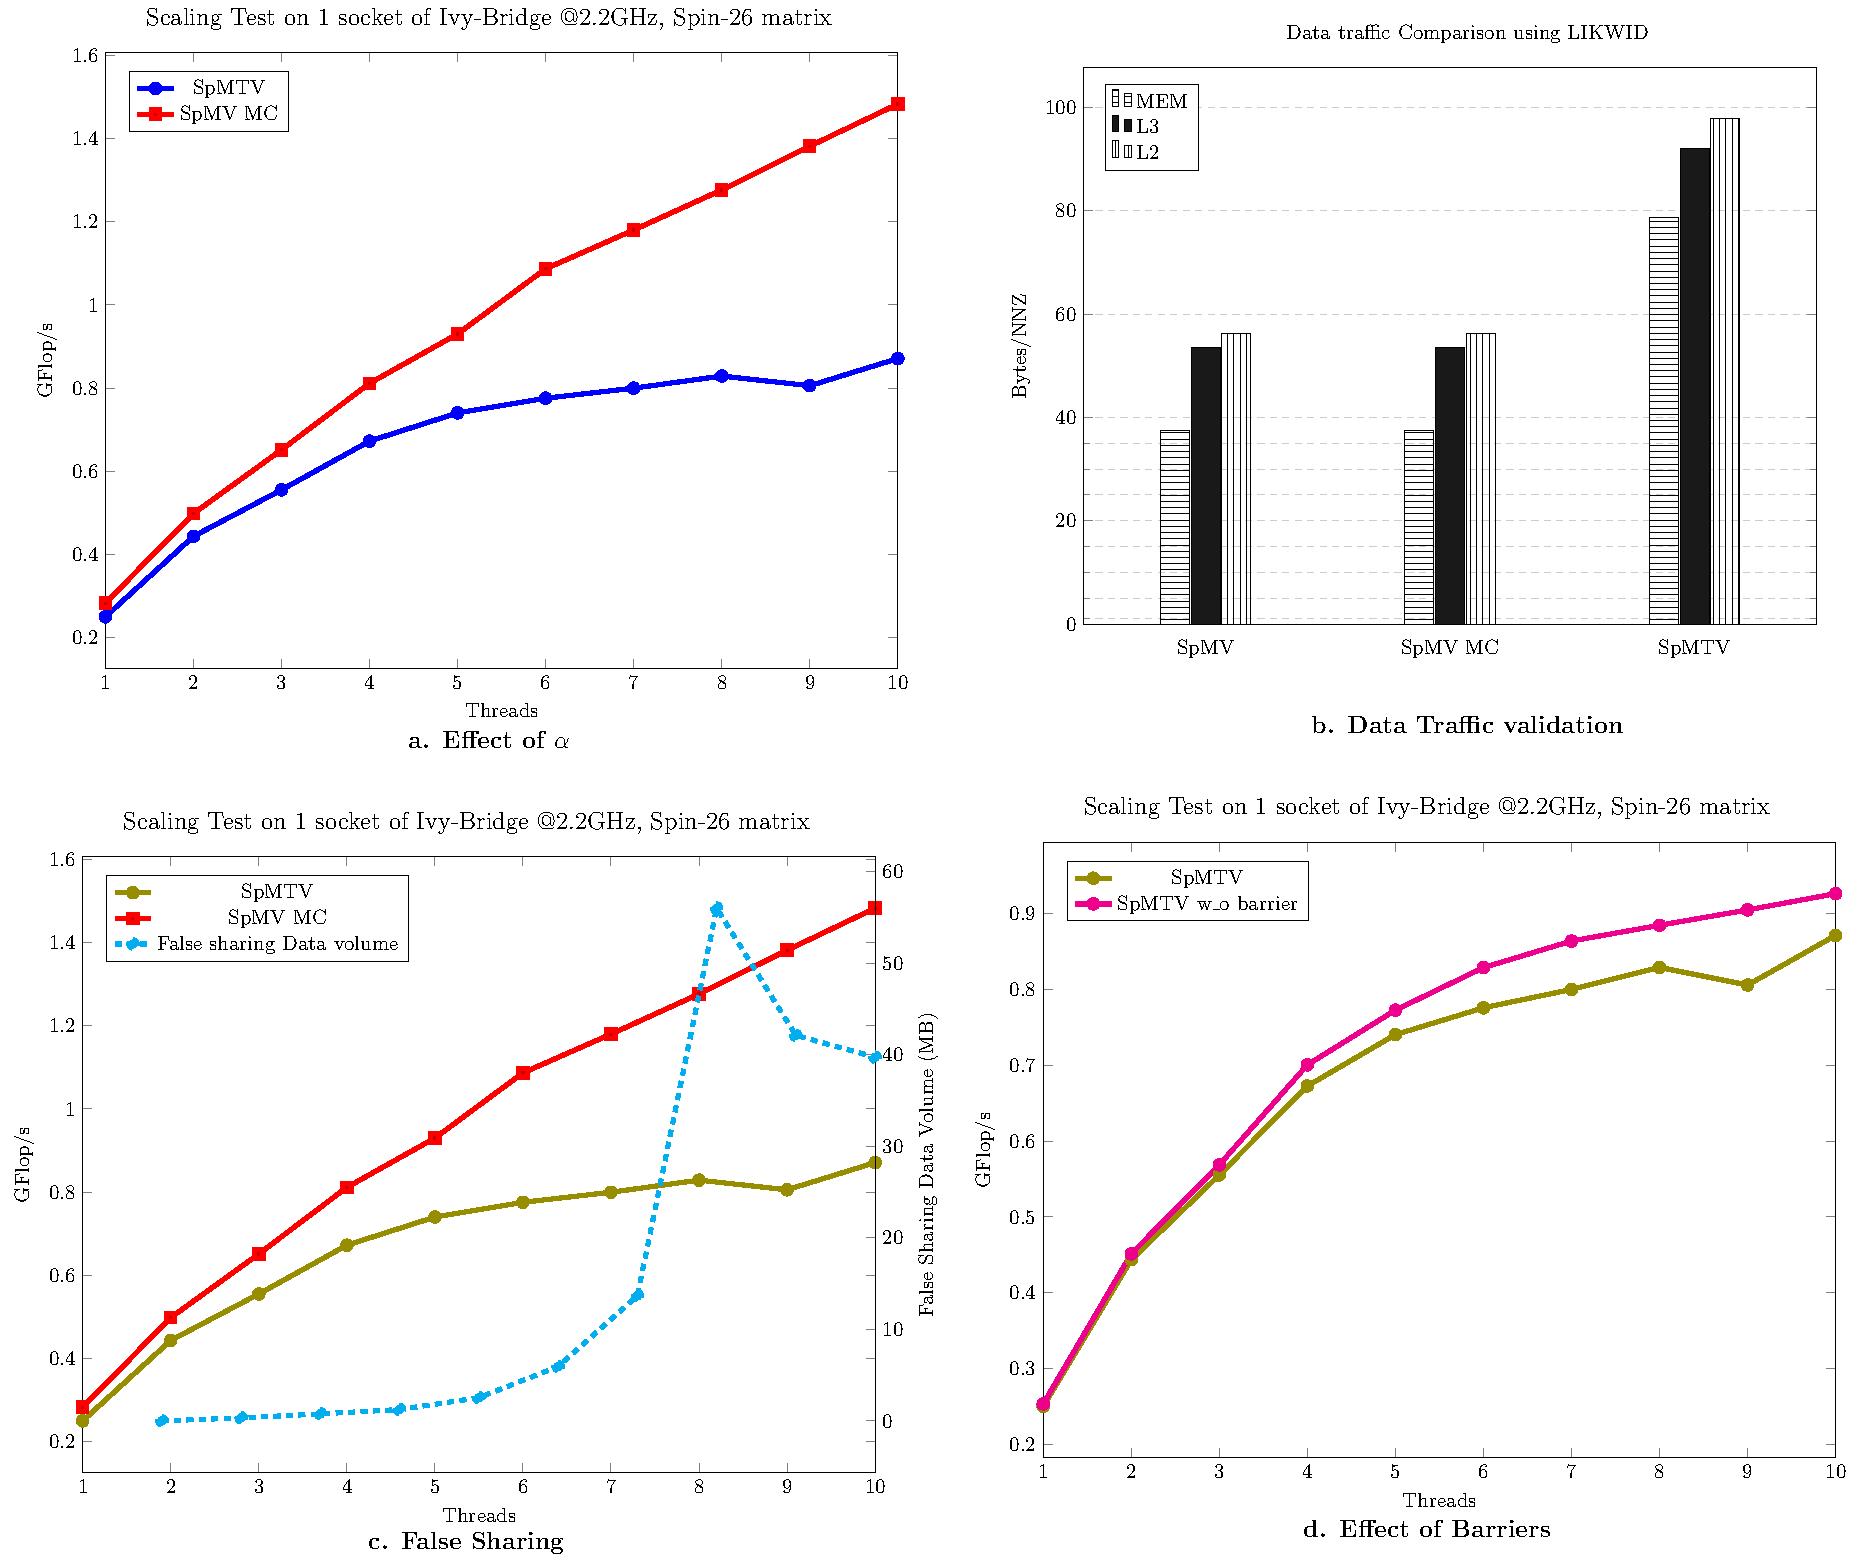
\includegraphics[width=0.9\textwidth, height=0.4\textheight]{pics/motivation/motivation}
  %	\caption{Illustration of increase in $\alpha$ by multicoloring, numbers represents thread numbers working on a particular row}
  %	\label{fig:motivation}
  %\end{figure}
  \begin{figure}[tbp]
  	\centering
  	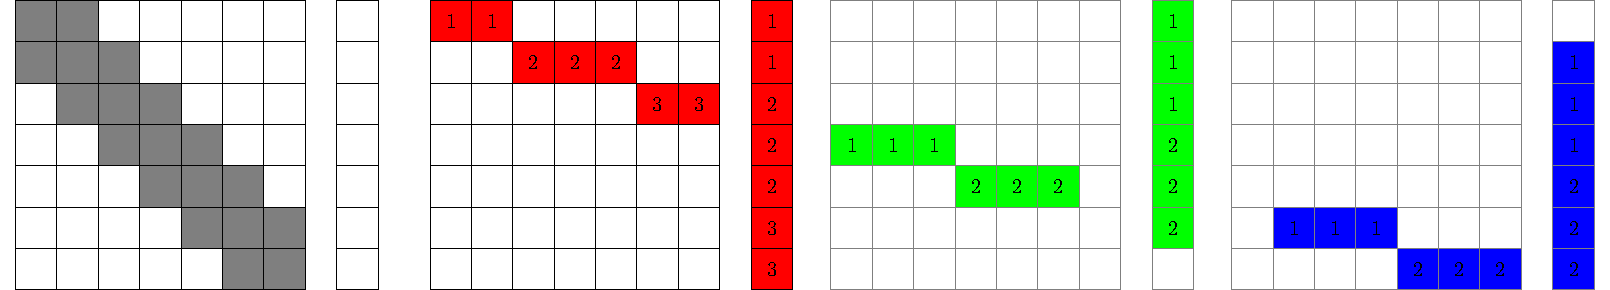
\includegraphics[scale=0.45]{pics/mc_alpha_problem/mc_alpha_unsymm}
  	\caption{Illustration of the increase of $\alpha$ by \acrshort{MC}. Numbers represent thread ids. Note that this figure shows only rows of the matrix permuted according to \acrshort{MC}, but in practice one would permute both rows and columns.}
  	\label{fig:mc_alpha}
  \end{figure}
  
The reason for this is the nature of the \acrshort{MC}
permutation. For \DTWO coloring, sets of structurally orthogonal
rows have to be determined \cite{dist_k_def}, \ie rows that do not
overlap in any column entry. These sets are referred to as colors. \Cref{fig:mc_alpha} shows the corresponding permutation
and the obtained sets of colors applied to a toy problem with high
data locality. Different rows of the same color can be executed in
parallel, but colors are operated one after the
other. After \acrshort{MC} a color may contain rows from very distant
parts of the matrix, potentially destroying data locality.  Assuming
that the \acrshort{LLC} can hold a maximum of six elements, we find
that the RHS vector must be loaded every time for each
new color. This is the reason why we observe 3$\times$ more bytes
per nonzero for \acrshort{SymmSpMV} with \acrshort{MC} compared
to \acrshort{SpMV}, as seen in~\cref{fig:motivation_data,fig:motivation_data_skx}.  However,
our performance model indicates that \acrshort{SymmSpMV} should
exhibit only 0.7$\times$ the data traffic of \acrshort{SpMV} (see
red dotted line in \cref{fig:motivation_data,fig:motivation_data_skx}). Of course this
effect strongly depends on the matrix structure, the matrix size, and
the cache size.
        
\Acrshort{ABMC}\cite{ABMC} tries to preserve data locality by first partitioning
the entire matrix into blocks of specified size and then
applying \acrshort{MC} to these blocks. Threads then work in parallel
between blocks of the same color. Along the lines of \cite{Park_HPCG} 
we use \METIS \cite{METIS} to partition the matrix into blocks, and COLPACK 
for \acrshort{MC}. The size of blocks for \acrshort{ABMC} is
determined by a parameter scan (range 4 \ldots 128;
see~\cite{ABMC})\@. As stated above, the timing for the performance measurements
excludes preprocessing and the parameter search. This method reduces the 
data traffic (see \cref{fig:motivation_data,fig:motivation_data_skx}) as there is better data
locality within a block. Consequently, the performance improves
over plain \acrshort{MC} (see \cref{fig:motivation_symm_spmv,fig:motivation_symm_spmv_skx}). However,
we are far off the performance model prediction. In
addition to data locality, other factors like global synchronizations
and false sharing also contribute to this failure. These
effects strongly depend on the number of colors and in general
increase with chromatic number. In the case of the Spin-26 matrix the overhead of
synchronization is roughly 10\% for the \acrshort{MC} method.  For most of
the matrices considered in this work one can also observe a strong
positive correlation between false sharing and the number of threads
for \acrshort{SymmSpMV} kernels due to the indirect writes
in \acrshort{SymmSpMV}.
 
 %As seen in \cref{fig:motivation_data} the data traffic further increases for \acrshort{SymmSpMV}, although ideally one would expect only half the data traffic as \\acrshort{SpMV} since we operate only with upper triangle part of the matrix. The reason for this extra traffic is due to additional indirect writes (scatter) and this scales up $\alpha$ factor as seen in the denominator of $I_{\acrshort{SymmSpMV}}$ (see \cref{eq:Symm\acrshort{SpMV}_intensity}),  which further decreases performance of \acrshort{SymmSpMV} compared to \\acrshort{SpMV} on \acrshort{MC} matrix. Note that ideal performance of \acrshort{SymmSpMV} is almost twice as that of \\acrshort{SpMV} if the code could saturate the memory bandwidth.
 


%Overall for all the matrix in our test-suite it was seen that average drop in performance by \acrshort{MC}full was almost a factor of two on a single socket of \IVB. Although for most of them performance could be improved by \acrshort{ABMC}full (\acrshort{ABMC}), still the results we obtained were not optimal (especially for large matrices) when compared to performance models which we will see later in \cref{Sec:expt}. This led to the development of a method which works on a common data format like \CRS in which most of the other kernels are written and at the same time preserves data locality, reduce synchronization overheads and false sharing. 

%In the following we address the above mentioned problems and formulate an improved hardware friendly coloring method called \acrshort{RACE} to alleviate these issues. This leads to substantial performance improvements, as seen in the case of Spin-26 matrix. Here we achieve close to optimal data traffic and a performance of 7.3 \GF(see \cref{fig:motivation}) which corresponds to 82 \% of our performance model using load-only bandwidth.

 

